\documentclass[12pt,lettersize,oneside]{article}
\usepackage[spanish]{babel}
\usepackage[utf8]{inputenc}
\usepackage{amsmath}
\usepackage{amssymb}
\usepackage{fancyhdr}
\usepackage{longtable}
\usepackage{listings}
\lstset{
  language=C,
  basicstyle=\small
}
\usepackage[pdftex]{graphicx}
\usepackage{color}
\definecolor{gray75}{gray}{.75}
\lstdefinestyle{consola}
{basicstyle=\small\bf\ttfamily,
backgroundcolor=\color{gray75},
}
\pagestyle{fancy}


\title{Primer versión de KECOSATS}
\author{Carlos Colmenares \and Kelwin Fernández \and Eleazar Leal}
\begin{document}
\maketitle
\setlength{\parskip}{2.5mm}
\setlength{\itemsep}{0ex }
%\tableofcontents
\section{Introducción}

\subsection{Motivación del proyecto}
En 1971, Stephen~Cook propuso en su trabajo\cite{Cook} una nueva categoría de complejidad
de problemas de decisión computacionales, a la que llamó problemas
\emph{NP-completos}. La caracterización de esta categoría se hace sobre estas
dos propiedades:
\begin{itemize}
  \item Todos los problemas \emph{NP-completos} pueden ser verificados en tiempo
    $O(p(n))$, donde $p(n)$ es un polinomio en función de $n$ el tamaño de la
    instancia del problema. 
  \item Todos los problemas en \emph{NP} pueden ser reducidos en tiempo
    $O(p(n))$ a algún problema \emph{NP-completo}, donde $p(n)$ es un polinomio
    en función de $n$ el tamaño de la instancia del problema que es reducido.
\end{itemize}

Ahora bien, fueron Cook y Leonid~Levin quienes encontraron, de forma
independiente, el primer problema en esta categoría \emph{NP-completos}: el
problema de la \emph{satisfacción booleana~(SAT)}. Un año después, Richard~Karp
identificó otros 21 problemas en esta categoría \cite{Karp}, los cuales tenían
la notoria característica de que para ellos no se conoce un algoritmo polinomial
(en función del tamaño de la instancia) que les dé solución, una cualidad que
comparten todos los problemas en esta clase, junto al hecho de que todos estos
problemas ocurren con una marcada frecuencia en el área de la computación. Sin
embargo, la característica más especial de éstos es el segundo ítem de arriba:
encontrar un algoritmo polinomial para tan sólo uno de ellos es encontrar un
algoritmo polinomial para todos.

De modo pues que la motivación para este proyecto estriba en el hecho de que
\emph{SAT} fue el primer problema que se demostró que pertenece a
\emph{NP-Completos} y que todos los problemas en esta clase son reducibles en
tiempo polinomial a él. Siendo así y bajo el supuesto de que estas reducciones a
\emph{SAT} se caractericen por polinomios de bajo grado y coeficientes pequeños,
cualquier mejora en tiempo que se pueda realizar a los algoritmos exponenciales
hoy conocidos para resolver el problema \emph{SAT} es una mejora para los
algoritmos exponenciales conocidos para los demás problemas en
\emph{NP-completos}.

\subsection{Breve descripción del problema} 
Llamaremos \emph{cláusula} a la disjunción de un conjunto finito de variables
booleanas, cada una de las cuales puede ocurrir con polaridad positiva (no
negada: $x_i$) o con polaridad negativa (negada $\overline{x_i}$).  
Ejemplos de cláusulas son: $(x_1 \wedge x_2)$, $(\overline{x_3})$,
$(\overline{x_1} \wedge x_3)$.

Una \emph{fórmula} es en cambio la conjunción de un conjunto finito de
cláusulas. Por ejemplo: $F_1:\ (x_1 \vee x_2 \vee \overline{x_3}) \wedge (x_1
\vee \overline{x_2}) \wedge (\overline{x_3})$ es una cláusula.

El \emph{problema de la satisfacción booleana~(SAT)} consiste de la
forma general de las instancias al problema y de la pregunta: \vspace{-2.5mm}
\begin{enumerate}
\item La forma general de las instancias: Dados un conjunto finito de variables
  booleanas $x_1,x_2,\ldots,x_n$ y una fórmula booleana $F(x_1,x_2,\ldots,x_n)$
  en forma normal conjuntiva (CNF).
\item La pregunta cuya respuesta se quiere determinar: ¿existe una asignación de
  valores de verdad a las variables $x_1,\ldots, x_n$ tal que la fórmula sea
  verdad?
\end{enumerate}

\subsection{Descripción del contenido del informe}
En el presente reporte se expondrán los algoritmos y tipos de datos
fundamentales empleados por el programa KECOSATS para decidir el problema de la
satisfacción booleana. Asimismo, se presentarán las decisiones de diseño que
orientaron la implementación del mismo.

\section{Diseño}

\subsection{Descripción general del algoritmo empleado}
El programa propuesto sigue el esquema general del algoritmo DPLL que presentaron
Martin Davis, Hilary Putnam, George Logemann y Donald Loveland para decidir el
problema de satisfacción booleana.

Seguidamente presentamos el esquema general del algoritmo DPLL, que hemos
adaptado de \cite{Zhang}:

\begin{lstlisting}
  status = preprocess(); 
if (status != UNKNOWN) return status; 
while(true) { 
  // Fase de seleccion de variable a asignar.
  decide_next_branch(); 
  while (true) { 
    // Fase de deduccion.
    status = deduce(); 
    if (status == CONFLICT) { 
      conflict_result = analyze_conflict(); 
      if (conflict_result == 0) 
        return UNSATISFIABLE; 
      else backtrack; 
    } 
    else if (status == SATISFIABLE) 
      return SATISFIABLE; 
    else break; 
  } 
 } 
\end{lstlisting}
\vspace{-2.5mm}

Uno de los puntos en que esta presentación del algoritmo diverge del que
presenta \cite{Zhang} es en el análisis de conflicto y en la posibilidad de
efectuar un \emph{backtracking} no cronológico. En el programa que aquí
describimos, no se realiza sino una versión muy simplificada de análisis de
conflicto, en donde no hay aprendizaje de cláusulas y el \emph{backtracking} se
hace sólo de un nivel de decisión en un nivel de decisión (cronológico).

Entre las razones por las que se escogió el algorimo DPLL están:
\begin{enumerate}
\item Este algoritmo es la base para las implementaciones de los
  \emph{SAT-solvers} completos ---no estocásticos--- más eficientes conocidos.
\item El esquema general del algoritmo es bastante sencillo de implementar como
  de comprender.
\end{enumerate}
\subsection{Fase de selección de variables a asignar}\label{ProxVariable}

En esta primera versión de KECOSATS se propone una heurística para la selección
de la próxima variable no asignada, a la que se le dará un valor booleano. La
heurística consiste en seleccionar entre todas las variables no asignadas hasta
el momento, a aquella variable ---sin importar la polaridad--- que aparezca como
\emph{watcher} o testigo en el mayor número de cláusulas posible. Ahora bien,
para seleccionar el valor de verdad que se va a asignar esta variable, se escoge
aquél valor que genere el mayor número de movimientos de \emph{watchers} en
todas las cláusulas.

La ventajas de haber escogido esta heurística son las siguientes:
\begin{enumerate}
\item En la mayoría de las instancias de pequeño tamaño en las que se probó esta
  heurística, se redujeron los tiempos de ejecución del programa.
\item La forma de escoger el valor a asignar a la variable, antes descrita,
  sugiere que pudiera ser más probable que se detecten con mayor rapidez los
  conflictos ---en caso de que los hubiera.
\item Se trata de una heurística muy sencilla de comprender e implementar.
\end{enumerate}

Como desventaja de esta heurística está que obviamente en el peor caso, habrá
que recorrer la lista completa de variables para encontrar aquel literal que
ocurre en el mayor número de cláusulas como \emph{watcher}.

\subsection{Fase de deducción}

Una vez que se ha seleccionado una variable para asignar junto al valor que se
le asignará, se inicia la fase de deducción del algoritmo DPLL. Es en esta fase
que se procede a la identificación y propagación de cláusulas unitarias. En esta
sección describiremos los algoritmos de propagación de restricciones booleanas y
de identificación y eliminación de literales puros.


\subsubsection{Identificación y propagación de cláusulas
  unitarias}\label{UnitPropagation}
Tal como se indica en \cite{Zhang} y \cite{ZhangThesis}, el estudio de
implementaciones del algoritmo DPLL que se han realizado con el pasar de los
años, sugiere que la propagación de cláusulas unitarias como mecanismo de
deducción parece ser el más eficiente que se ha encontrado hasta ahora.

La \emph{propagación de cláusulas unitarias} consiste en ubicar cuáles cláusulas
de la fórmula ---dada ésta en forma normal conjuntiva--- están compuestas de un
solo literal. Estas cláusulas son llamadas \emph{cláusulas unitarias} y se
satisfacen con asignar a éste único literal el valor de verdad correspondiente.
Lo explicamos con un ejemplo: En la fórmula $F_1:\ (x_1 \vee x_2 \vee
\overline{x_3}) \wedge (x_1 \vee \overline{x_2}) \wedge (\overline{x_3})$, la
única cláusula unitaria es $\overline{x_3}$. Si se asigna $x_3:=0$, queda la
nueva fórmula $F_2:\ (x_1 \vee x_2 \vee \overline{x_3}) \wedge (x_1 \vee
\overline{x_2}) $ y bajo el supuesto de que $x_3=0$ se tiene que $F_2$ es
satisfactible si y sólo si $F_1$ lo es.

La implementación de la propagación de cláusulas unitarias con 2 testigos por
cláusula (\cite{Zhang} y \cite{ZhangThesis} los llama \emph{2-watched literals})
empleada por \emph{zChaff} asocia a cada literal $x_i,\ i\in{1,\ldots,n}$ un par
de listas, la primera de ellas tiene como elementos a todas las cláusulas en las
que la el literal $x_i$ ocurre no negado (polaridad positiva) como testigo o
\emph{watched literal}. La segunda lista asociada a $x_i$ tiene como elementos a
todas las cláusulas en las que el literal $\overline{x_i}$ ocurre como testigo o
\emph{watched literal}.

Asimismo, cada cláusula tiene asociados dos apuntadores a literales que ocurren
dentro de ella, estos apuntadores son los \emph{watchers} a los que nos hemos
referido antes.

Ahora bien, para detectar si, tras asignar $x_i=0$, una cláusula
es unitaria se buscan todas las cláusulas en las que aparezca $x_i$ con
polaridad positiva (no negada) y como \emph{watcher}. Este último apuntador debe
ser movido a otro literal no asignado en la misma cláusula. Si el único literal
no asignado en esa cláusula está siendo apuntado por el otro \emph{watcher}
entonces esa cláusula es unitaria. 

Para la implementación de este mecanismo de deducción, se escogió la
implementación de los \emph{2-watched literals} descrita en las fuentes
\cite{Marques}, \cite{Zhang} y \cite{ZhangThesis} y que fue propuesta con el
programa \emph{Chaff}.

% Seguidamente describiremos someramente la implementación \emph{2-watched
%   literals} para la detección de cláusulas unitarias. Sin embargo, referimos al
% lector a los trabajos \cite{Marques}, \cite{Zhang} y \cite{ZhangThesis} para una
% explicación más detallada.


Las razones para escoger esta implementación de \emph{2-watched literals} para
la identificación de cláusulas unitarias son las siguientes:\vspace{-2.5mm}
\begin{enumerate}
\item En pruebas de ejecución\cite{Zhang} se ha observado que el comportamiento
  de la implementación por \emph{2-watched literals} requiere de menor tiempo
  que implementaciones como la de \emph{SATO} ---implementación a la que
  \cite{Zhang} se refiere como \emph{Head/Tail lists}--- y considerablemente
  menor tiempo que la implementación por contadores.
\item La implementación de \emph{2-watched literals} no requiere que se realicen
  operaciones sobre los \emph{watchers}, o sobre el conjunto de datos que
  permite directamente determinar cuáles son las cláusulas unitarias, cuando se
  realiza el \emph{backtracking} a un nivel de decisión anterior. Las
  implementaciones de \emph{SATO} y contadores sí requieren estas
  operaciones. Esta ventaja es señalada por el trabajo \cite{Marques}.
\end{enumerate}

Entre las desventajas que trae consigo la implementación de \emph{2-watched
  literlas} está:\vspace{-2.5mm}
\begin{enumerate}
\item Cuando es necesario mover alguno de los \emph{watchers}, porque la variable
  a la que apuntan en la cláusula resulta asignada, se debe buscar una nueva
  variable no asignada---puede que ni exista tal variable--- en la misma
  cláusula. Entonces, en el peor caso, para identificar una cláusula unitaria,
  la implementación de \emph{2-watched literals} tendrá que \emph{recorrer todos
    los literales de una misma cláusula} en busca de esta variable no asignada.
\end{enumerate}



\subsubsection{Eliminación de literales puros}

La \emph{eliminación de literales puros} en una fórmula dada en forma normal
conjuntiva consiste en ubicar primero cuáles son las variables booleanas que
sólo ocurren con una polaridad en la fórmula. Ahora bien, estos literales que
ocurren con una única polaridad en toda la fórmula no condicionan la
satisfacción de la fórmula; es decir, si se eliminaran todos los literales
puros, la fórmula resultante es satisfactible si y sólo si asignando a los
literales puros los valores de verdad que los satisfagan, se logra que la
fórmula original lo sea. Lo explicamos con un ejemplo: En la fórmula siguiente
$F_1:\ (x_1 \vee x_2 \vee \overline{x_3}) \wedge (x_1 \vee \overline{x_2})
\wedge (\overline{x_3})$ el único literal puro es $x_1$, de forma que $F_1$ será
satisfactible si y sólo si asignando a $x_1$ el valor de verdad se logra que
$F_2:\ (x_2 \vee \overline{x_3}) \wedge (\overline{x_2}) \wedge
(\overline{x_3})$ sea satisfecha.

Para la implementación de este mecanismo de deducción se hizo un recorrido por
todas las cláusulas de la fórmula anotando cuál es la polaridad que se ha
observado para cada literal. Si en un momento del paseo por las cláusulas de la
fórmula se encuentra con un literal que ocurre con una polaridad distinta a la
ya observada anteriormente para ese literal, se descarta que esa variable sea un
literal puro. Para más detalles consultar más adelante.

\section{Implementación}

El programa que proponemos está orientado por los cambios que se efectúan,
durante la ejecución, sobre una variable global de nombre {\tt sat\_st} que es la
única con el tipo {\tt SAT\_status} en todo el programa. 
Este tipo de dato registra: \vspace{-4.5mm}
\begin{enumerate}
\item La información que es necesario preservar de la instancia del problema de
  satisfacción que se ha leído y que se pretende resolver.
\item El estatus de resolución de un problema de satisfacción en cualquier
  momento dado.
\end{enumerate}
Por esta razón podríamos afirmar que este es el tipo de dato más importante de
todo el programa.
Presentamos ahora la definición del tipo {\tt SAT\_status}
\begin{lstlisting}
typedef struct SAT_status{    
    int num_vars;
    int num_clauses;
    clause *formula;
    list *pos_watched_list;
    list *neg_watched_list;
    stack backtracking_status;
    int *model;                     
} SAT_status;
\end{lstlisting}
, para comentar sus campos con detalle:\vspace{-2.5mm}
\begin{itemize}
\item El atributo {\tt formula}, representa la fórmula en forma normal
  conjuntiva. Se trata de un arreglo de cláusulas, cada una de tipo {\tt
    clause}.
\item En la implementación que aquí se describe, se optó por por los campos {\tt
    pos\_watched\_list} y {\tt neg\_watched\_list} en el tipo {\tt
    SAT\_status}. Cada uno de éstos es un arreglo de cabezas de listas, de forma
  que {\tt pos\_watched\_list[i]} sea la cabeza de la lista cuyos elementos son
  las cláusulas en las que el literal $x_i$ ocurre como
  \emph{watcher}. Análogamente ocurre con {\tt neg\_watched\_list[i]}: es la
  cabeza de la lista cuyos elementos son las cláusulas en las que el literal
  $\overline{x_i}$ ocurre como \emph{watcher}.

\item El campo {\tt model} del tipo {\tt SAT\_status} es un arreglo de enteros
  tal que {\tt model[i]} es el valor de asignación que se prueba para la
  variable $x_i$. El {\tt model} indica cuál nodo de la arborescencia del
  \emph{backtracking} se está considerando en un determinado instante de la
  ejecución\footnote{Véase la sección \ref{backtracking} que describe la
    arborescencia implícita que se recorre en el \emph{backtracking}.}.

\item Se incluye el campo {\tt num\_clauses} en el tipo {\tt SAT\_status}, para
  poder recorrer el arreglo {\tt formula} de todas las cláusulas que componen la
  fórmula.
\end{itemize}

A continuación comentaremos algunos detalles sobre la variable global {\tt
  sat\_st}. La razón por la que se escogió a {\tt sat\_st} de tipo {\tt
  SAT\_status} como variable global, en lugar de pasarla como parámetro entre
las sucesivas llamadas a funciones durante la ejecución del algoritmo son:
\begin{enumerate}
\item El pasaje del parámetro {\tt sat\_st} a cada una de las funciones supone
  un costo acumulado muy grande a lo largo de la ejecución de todo el
  programa. Cuando bien pudiera ahorrarse la operación de empilar esa parámetro
  en cada llamada.
\item Si se pasara una referencia a {\tt sat\_st} como parámetro a cada función,
  se incurriría en un costo adicional, en comparación con la alternativa de
  tener a {\tt sat\_st} como variable global, por la indirección que es
  necesario ejecutar en cada subrutina por cada vez que se quiera acceder a los
  campos de esta variable.
\end{enumerate}

\subsection{Implementación de las cláusulas}\label{clausulas}

Para la implementación de cada cláusula se definió el siguiente tipo de dato
{\tt clause}:
\begin{lstlisting}
typedef struct clause{
    int size;
    variable* head_watcher;
    variable* tail_watcher;
    variable* literals;
} clause;
\end{lstlisting}
, que a continuación describiremos campo por campo.\vspace{-2.5mm}
\begin{enumerate}
\item Los apuntadores {\tt head\_watcher} y {\tt tail\_watcher} señalan cuáles
  son los literales testigos ---\emph{watched literals}--- de una cláusula. En
  virtud de que en la fase de propagación de restricciones booleanas se optó por
  implementar la propagación de cláusulas unitarias con los \emph{2-watched
    literals} según se describe en \cite{Zhang},
  cada cláusula exige dos apuntadores a variables en la misma cláusula.

\item Como cada cláusula es una disjunción de literales, optamos por
  representarla como un arreglo de variables llamado {\tt literals}. Para poder
  recorrerlo es necesario almacenar su tamaño, que estará almacenado en el campo
  {\tt size} de la cláusula.
\end{enumerate}

\subsubsection{Ventajas de la implementación escogida para las cláusulas}
La implementación de los literales que componen una cláusula en un arreglo de
variables apuntado por {\tt literals} implica: \vspace{-2.5mm}
\begin{itemize}
\item Una rapidez de acceso en tiempo constante a cada literal de la
  cláusula. Hecho que resulta de particular utilidad en los recorridos a través
  de los literales de cada cláusula que son efectuados durante la detección de
  literales puros y durante la actualización de los \emph{watchers} o testigos
  que permiten identificar cláusulas unitarias. 

  Recuerde el lector que se ha mencionado en la sección \ref{UnitPropagation} que
  una de las desventajas de las implementación por \emph{2-watched literals} es
  que en el peor caso hay que recorrer todos los literales de una cláusula para
  determinar si ésta es unitaria o no.

\item Un ahorro de espacio para los apuntadores, el cual sería necesario si la
  conjunción de literales en las cláusulas se implementara con una lista
  enlazada.
\end{itemize}

\subsection{Implementación del \emph{Backtracking}}
\subsubsection{\'Arbol implícito del \emph{Backtracking}}\label{backtracking}
Toda implementación de \emph{Backtracking} es un recorrido \emph{Depth-First
  Search} sobre una arborescencia implícita. Esta descripción implícita de la
arborescencia a recorrer exige que se defina cuáles son sus nodos y para cada
nodo, cuáles son sus nodos sucesores. En el caso que nos concierne, los nodos
son de la forma:
\[[x_{i_1}=\mathbb{B},x_{i_2}=\mathbb{B},\ldots, x_{i_k} = \mathbb{B} ], \]
donde $0\leq k \leq n$, con $n$ el número de variables de la instancia del
problema de satisfacción a resolver y $x_{i_k}=\mathbb{B}$ indica que la
variable booleana $x_{i_k}$ tiene un valor booleano (sea $1$ ó $0$)
asignado. Imponemos adicionalmente una condición a los nodos de esta
arborescencia y es que la asignación hecha a las variables del nodo:
$x_{i_1},\ldots,x_{i_k}$ \emph{no haga que la fómula no se pueda
  satisfacer}. Las $x_{i_k}$ denotan variables booleanas distintas $\forall k
\in \{1,\ldots,n\}$.

Ahora, dado un nodo $[x_{i_1}=\mathbb{B},x_{i_2}=\mathbb{B},\ldots, x_{i_k} =
\mathbb{B} ]$ sus sucesores son todos los nodos de la forma:
$[x_{i_1}=\mathbb{B},x_{i_2}=\mathbb{B},\ldots, x_{i_k} = \mathbb{B},
x_{i_{k+1}}=\mathbb{B} ]$.

El \emph{backtracking} implementado busca encontrar en la arborescencia ---en
caso de que exista--- un nodo de la forma
\[[x_{1}=\mathbb{B},x_{2}=\mathbb{B},\ldots, x_{n} = \mathbb{B} ], \] y que se
corresponde con una asignación de valores de verdad a todas las variables que
hace que la fórmula dada sea satisfecha ---si $n$ es el número total de
variables booleanas.
\vspace{-2.5mm}

\subsubsection{Estructuras de datos que apoyan la implementación del \emph{bactracking}}
El \emph{backtracking} se implementó iterativo en lugar de recursivo, por los
motivos que se señalan en la sección \ref{VentajasBacktracking}. Para ello fue
necesario trabajar explícitamente con una pila de elementos de un nuevo tipo de
dato llamado {\tt decision\_level\_data}. Este tipo almacena la información que
caracterizan a cada nodo del árbol implícito que se recorre en el
\emph{backtracking}\footnote{En \cite{Zhang} les llaman niveles de decisión.} y
que deben ser conservados en caso de que el algoritmo se encuentre con un nodo
parcial que no tiene sucesores; esto es, con un nodo
$[x_{i_1}=\mathbb{B},x_{i_2}=\mathbb{B},\ldots, x_{i_k} = \mathbb{B} ]$, $k< n$
tal que la asignación de cualquier otra variable no logra satisfacer la fórmula.

Presentamos entonces el tipo {\tt decision\_level\_data}:

\begin{lstlisting}
typedef struct decision_level_data{
    variable assigned_literal;
    int missing_branch;                                                
    list propagated_var;
} decision_level_data;
\end{lstlisting}
que a continuación describimos:
\vspace{-2.5mm}
\begin{enumerate}
\item El campo {\tt assigned\_literal} contiene el valor y el nombre del literal
  asignado en un determinado nivel de decisión. Expresado de otra forma,  si
  $[x_{i_1}=\mathbb{B},x_{i_2}=\mathbb{B},\ldots, x_{i_k} = \mathbb{B} ]$, $k< n$, $v_k
  \in \mathbb{B}$ es un nodo de la arborescencia recorrida con el
  \emph{backtracking}, en el momento en que se consideran una nueva variable
  $x_{i_{k+1}}$ con un valor booleano se ha creado un nuevo nivel de decisión
  caracterizado por un elemento del tipo {\tt decision\_level\_data} en el
  programa. Este elemento tendrá en su campo {\tt assigned\_literal} a la
  variable $x_{i_{k+1}}$ con su valor.
\item El campo {\tt missing\_branch} es un valor booleano que es cierto si y
  sólo si se ha explorado la asignación de {\tt assigned\_literal} con un
  sólo valor de verdad. Es decir, si
  $[x_{i_1}=\mathbb{B},x_{i_2}=\mathbb{B},\ldots, x_{i_k} = v_k ]$, $k< n$, $v_k
  \in \mathbb{B}$ es un nodo de la arborescencia recorrida con el
  \emph{backtracking}, en la que la variable $x_{i_k}$ fue la última variable
  asignada con un valor booleano determinado, {\tt missing\_branch} será cierto
  si y sólo si el conjunto de asignaciones
  $[x_{i_1}=\mathbb{B},x_{i_2}=\mathbb{B},\ldots, x_{i_k} = \overline{v_k} ]$,
  $k<n$ \emph{todavía no ha sido estudiado} si es nodo o no.
\item El campo {\tt propagated\_var} es la cabeza de una lista cuyos elementos
  son todas las variables booleanas cuya asignación actual se dedujo a partir de
  la propagación de cláusulas unitarias que aparecen en la fórmula como
  consecuencia de la asignación del {\tt assigned\_literal}.
\end{enumerate}

\subsubsection{Ventajas de la implementación escogida para el
  \emph{backtracking}}\label{VentajasBacktracking}
Entre las ventajas de la implementación iterativa para el \emph{backtracking} está:
\vspace{-2.5mm}
\begin{itemize}
  \item Resultará más sencillo modificar el programa para implementar un
    \emph{bactracking} no cronológico, que si se hubiera implementado el
    \emph{backtracking} de manera recursiva.
\end{itemize}

\subsubsection{Desventajas de la implementación escogida para el \emph{backtracking}}
Quizás la única desventaja de la implementación iterativa respecto a la
recursiva para el \emph{backtracking} sea la mayor dificultad que supone el
manejo explícito de la pila, que en el caso recursivo se maneja implícitamente
con la pila de llamadas a subrutinas.


%\subsection{Problemas encontrados y la manera como fueron resueltos}
\section{Implementación de Propagación de Cláusulas Unitarias.}
Como se mencionó en la sección \ref{UnitPropagation}, el algoritmo empleado para
la detección y propagación de cláusulas unitarias es el de los \emph{2-watched
  literals}, que fue propuesto por los desarrolladores del programa
\emph{zChaff}. Ahora bien, nuestra implementación del algoritmo no difiere de la
que se encuentra descrita en \cite{Zhang}. En la sección \ref{clausulas}
comentamos acerca del par de \emph{watchers} que tiene asociados cada cláusula y
anteriormente comentamos también sobre los arreglos de cabezas de listas {\tt
  pos\_watched\_list} y {\tt neg\_watched\_list}, tales que  {\tt
  neg\_watched\_list[i]} es la cabeza de la lista de cláusulas en las que el
literal $x_i$ ocurre de la forma $\overline{x_i}$ como watcher.

Una vez comentado esto y en virtud de que nuestra implementación de la
propagación de cláusulas unitarias no difiere de la expuesta en \cite{Zhang},
consideramos que no hay nada más que agregar al respecto.

\section{Dificultades encontradas}
Entre las dificultades encontradas a lo largo del desarrollo de esta primera
versión de KECOSATS están:
\begin{itemize}
\item El problema del manejo de la memoria: En varios puntos del programa se
  emplean listas enlazadas para implementar pilas. Así que todas las operaciones
  de empilamiento ejecutan llamadas al sistema que consumen mucho tiempo. En
  esta primera entrega se decidió mantener esta implementación de pilas que
  realizan llamadas al sistema en cada {\tt push} por el motivo de su
  sencillez. Se dice ``sencillez'' porque para evitarse estas llamadas al
  sistema KECOSATS tendría que tener su propio manejador de memoria.
\item El problema de la selección de la próxima variable a asignar. En un
  principio se consideró como algoritmo de selección de variables el siguiente:
  se supone que las variables $x_1,x_2,\ldots,x_n$ de la instancia están
  ordenadas. Se selecciona la variable $x_i$ con el índice $i$ menor entre todas
  las variables que no han sido asignadas. Como se tiene almacenada la última
  variable asignada y una vez asignada una variable ésta permanece asignada, la
  selección de la próxima variable tarda un tiempo constante. Al observar con
  algunas instancias pequeñas que KECOSATS se demoraba un poco, se decidió
  sustituir este algoritmo por el que se describió en la sección
  \ref{ProxVariable}, logrando con ello mejorar el desempeño del programa.
\end{itemize}

\section{Instrucciones de operación}
Para emplear la aplicación, escribir en la consola el comando
\begin{lstlisting}[style=consola]
# kec_o_sat_s -f inputfilename -o outputfilename 
\end{lstlisting}
\noindent donde:
\vspace{-2.5mm}
\begin{itemize}
\item {\tt inputfilename} es el nombre del archivo que contiene la instancia del
  problema SAT a resolver. Esta instancia debe estar en el formato DIMACS.
(Consultar http://logic.pdmi.ras.ru/~basolver/dimacs.html para información sobre
este formato.)
\item {\tt outputfilename} es el nombre del archivo que contendrá los resultados
  generados tras correr el algoritmo.
\end{itemize}

Para más detalles acerca de la operación, leer el archivo {\tt README} que se
incluye con la distribución del programa.
\section{Estado Actual}
El programa se encuentra totalmente operativo.

\section{Comparación de desempeño entre KECOSATS y zChaff}

Tras ejecutar $60$ casos de prueba
\footnote{http://www.ldc.usb.ve/\%7Emeza/ci-5651/e-m2011/InstanciasSudoku.txt},
cada uno una instancia de SUDOKU que es transformada a una instancia equivalente
de SAT, en un computador Intel Core 2 Duo, 2.4Ghz con 4Gb de memoria RAM
corriendo en la distribución Ubuntu 10.04, se
obtuvieron los siguientes resultados:

Nota 1: Un tiempo de $-1$ segundos en la columna de tiempos para KECOSATS indica que
este programa, para esa instancia de SUDOKU (transformada a SAT), se demoró más
de $6$ minutos en dar una respuesta.

Nota 2: Los tiempos en negrillas en la columna de tiempos para KECOSATS indica
que este programa, para esa instancia de SUDOKU (transformada a SAT) se
desempeñó mejor que zChaff en tiempo.

\begin{longtable}{c|c}
\textbf{Tiempo ZChaff} (segundos) & \textbf{Tiempo KECOSATS} (segundos) \\\hline
0.0201 & \textbf{0.0173} \\
0.0256 & -1.0000 \\
0.0456 & -1.0000 \\
0.0209 & \textbf{0.0176} \\
0.0205 & 0.0236 \\
0.0209 & \textbf{0.0173} \\
0.0213 & 0.0247 \\
0.0201 & 0.0206 \\
0.0209 & \textbf{0.0181} \\
0.0439 & -1.0000 \\\hline
0.0211 & \textbf{0.0208} \\
0.0198 & \textbf{0.0186} \\
0.0266 & \textbf{0.0186} \\
0.0388 & -1.0000 \\
0.0411 & -1.0000 \\
0.0229 & \textbf{0.0177} \\
0.0281 & \textbf{0.0200} \\
0.0445 & -1.0000 \\
0.0208 & \textbf{0.0175} \\
0.0338 & -1.0000 \\\hline
0.0212 & \textbf{0.0172} \\
0.0293 & \textbf{0.0199} \\
0.0221 & -1.0000 \\
0.0262 & -1.0000 \\
0.0261 & -1.0000 \\
0.0264 & -1.0000 \\
0.0214 & -1.0000 \\
0.0338 & -1.0000 \\
0.0207 & 0.0219 \\
0.0309 & \textbf{0.0248} \\\hline
0.0247 & \textbf{0.0165} \\
0.0210 & 0.1374 \\
0.0531 & -1.0000 \\
0.0369 & -1.0000 \\
0.0295 & -1.0000 \\
0.0234 & -1.0000 \\
0.0210 & \textbf{0.0184} \\
0.0231 & 45.6845 \\
0.0251 & -1.0000 \\
0.0331 & 0.1749 \\\hline
0.0209 & \textbf{0.0188} \\
0.0242 & \textbf{0.0176} \\
0.0688 & -1.0000 \\
0.1071 & 0.1159 \\
0.0704 & \textbf{0.0628} \\
0.0657 & \textbf{0.0503} \\
0.0800 & -1.0000 \\
0.0256 & 0.0440 \\
0.0254 & \textbf{0.0204} \\
0.0218 & 0.0249 \\\hline
0.0244 & \textbf{0.0192} \\
0.0255 & \textbf{0.0218} \\
0.0320 & 0.0399 \\
0.0334 & \textbf{0.0175} \\
0.0393 & \textbf{0.0204} \\
0.0337 & \textbf{0.0242} \\
0.0310 & -1.0000 \\
0.0209 & \textbf{0.0177} \\
0.0209 & \textbf{0.0174} \\
0.0208 & 0.0274 \\ \hline
\end{longtable}


Más abajo se incluye una gráfica que permitirá captar más fácilmente las diferencias en el rendimiento entre estos dos programas:
\begin{center}
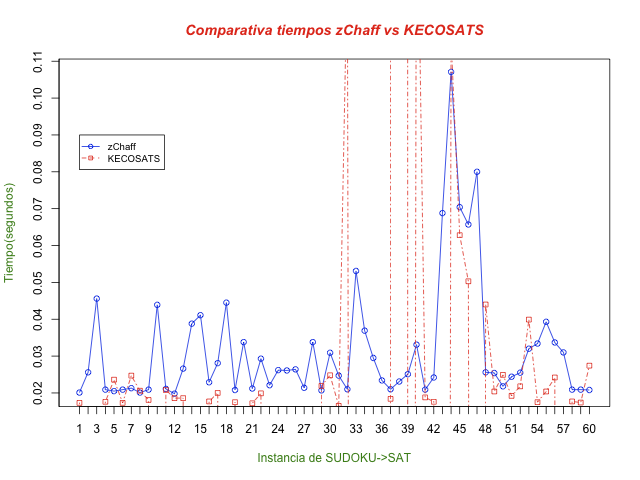
\includegraphics[scale=0.6]{compare.png}
\end{center}

Comentarios acerca de los resultados obtenidos, expuestos gráficamente en la ilustración de arriba:\vspace{-2.5mm}
\begin{itemize}
\item En 27 de los 60 casos de prueba (cerca del 50\% de los casos), KECOSATS
  tiene un rendimiento \emph{ligeramente mejor} que zChaff. En estos casos, las
  diferencias de tiempo entre KECOSATS y zChaff son algunas centésimas de
  segundo.
\item En 11 de los 60 casos de prueba (cerca del 15\% de los casos), KECOSATS
  tiene un rendimiento \emph{ligeramente peor} que zChaff. En estos casos, las
  diferencias de tiempo entre KECOSATS y zChaff son algunas centésimas de
  segundo.
\item En 1 de los 60 casos de prueba (cerca del 2\% de los casos), KECOSATS
  tiene un rendimiento \emph{peor} que zChaff. En este caso, la diferencia de
  tiempo entre KECOSATS y zChaff es de unos 45 segundos, cuando zChaff da la
  respuesta en fracciones de segundo.
\item En 21 de los 60 casos de prueba (cerca del 30\% de los casos), la demora
  de KECOSATS en dar una solución es superior a los 6 min, cuando zChaff da
  resultados en fracciones de segundo.
\end{itemize}

\section{Conclusiones y recomendaciones}

A continuación se comentará sobre algunas recomendaciones para KECOSATS.

En esta primera versión de KECOSATS hay varios aspectos que pudieran ser
modificados para obtener un mejor desempeño. Entre los aspectos que podemos
citar están:
\begin{itemize}
\item El manejo de la memoria. En varios puntos del programa es necesario armar
  listas de elementos y estas operaciones implican llamadas al sistema para la
  solicitud de memoria. Demás está decir el tiempo que consumen estas peticiones
  al sistema operativo. Se propone para la próxima entrega que KECOSATS
  incorpore su propio manejador de memoria, que solicite al arrancar un gran
  trozo de memoria y se encargue él solo de la gestión de este recurso,
  ahorrando así el tiempo que se consumen las llamadas {\tt malloc}. Ahora bien,
  es conocido por los desarrolladores que la realización de un manejador de
  memoria de ``buen desempeño'' no es algo trivial, particularmente si los
  segmentos de memoria que se solicitaría el programa a sí mismo pueden tener
  cualquier tamaño en algún rango dado. No obstante, dada la naturaleza de los
  elementos en las listas, los bloques de memoria que el programa se solicitaría
  a su propio manejador serían prácticamente homogéneos en cuanto al tamaño, lo
  cual facilitaría la tarea de programación de este manejador.
\item El problema de la selección de la próxima variable, al que nos hemos
  referido anteriormente en varias oportunidades. La mejora en los tiempos de
  ejecución de KECOSATS, producto del algoritmo implementado, que consiste en
  seleccionar la variable que apareza en el mayor número de cláusulas como
  \emph{watcher}, nos inclina a conjeturar que es posible que otras heurísticas
  igualmente sencillas puedan producir resultados aún mejores. Es conveniente
  por ello consultar un poco más a fondo sobre estos algoritmos de selección de
  variables en fuentes como \cite{Zhang} y \cite{ZhangThesis}, en las que se
  comenta sobre heurísticas como la  \emph{Variable State Independent Decaying
    Sum (VSIDS)}. Sería recomendable considerar mejorar la heurística para una
  segunda versión de KECOSATS.
\end{itemize}

Como conclusión de los resultados obtenidos tras la comparación de la demora de
KECOSATS y la de zChaff para resolver los 60 casos de prueba, concluimos que el
rendimiento de KECOSATS es aceptable para esta primera versión del programa
porque el 67\% de los casos de prueba dieron resultados en un tiempo
razonable. No obstante, la demora de más de 6 minutos para el 30\% de los casos
probados es un asunto en el que hay que trabajar con más cuidado. Consideramos
entonces que las mejoras propuestas en el apartado de arriba merecen especial
consideración, con el objetivo de disminuir los tiempos de este 30\% de los
casos.

\begin{thebibliography}{99}
\bibitem{Cook}Cook, Stephen: ``The complexity of theorem-proving
  procedures''. \emph{ACM}, 1971.
\bibitem{Karp}Karp, Richard: ``Reducibility Among Combinatorial
  Problems''. \emph{Complexity of Computer Computations}. 1972.
  . \emph{ACM}, 1971.
\bibitem{Marques}Lynce, I. y Marques-Silva, J.: ``Efficient Data Structures for
  Fast SAT Solvers''. Reporte Técnico. \emph{Cadence European Laboratories,
    Instituto de Engenharia de Sistemas e Computadores}. 2001.
\bibitem{Zhang}Zhang, Lintao y Malik, Sharad: ``The Quest for Efficient Boolean
  Satisfiability Solvers''.
\bibitem{ZhangThesis}Zhang, Lintao: ``Searching for truth: Techniques for
  satisfiability of boolean formulas''. \emph{Tesis de doctorado. Princeton
    University}. 2003.
\end{thebibliography}

\end{document}
